%%%%%%%%%%%%%%%%%%%%%%%%%%%%%%%%%%%%%%%%%%%%%%%%%%%%%%%%%%%%%%%
%
% University of Milano Bicocca
% Software engineering project
% Developed by
% 
% 
% 
% Tasca Alessandro 845150
% Lenzini Giacomo 854626
% Bonfanti Samuele 851656
% Dedo' Shana 851660
% 
% 
%
%%%%%%%%%%%%%%%%%%%%%%%%%%%%%%%%%%%%%%%%%%%%%%%%%%%%%%%%%%%%%%%

\documentclass[12pt]{article}

% Language setting
\usepackage[italian]{babel}

% Set page size and margins
% Replace `letterpaper' with`a4paper' for UK/EU standard size
\usepackage[letterpaper,top=2cm,bottom=2cm,left=3cm,right=3cm,marginparwidth=1.75cm]{geometry}

% Useful packages
\usepackage{float}
\usepackage{amsmath}
\usepackage{graphicx}
\usepackage[colorlinks=true, allcolors=green]{hyperref}


\title{
  Brew Day! \\ 
  \large Ingengeria del Software \\
    aa 2021-2022}

\author{Tasca Alessandro, Lenzini Giacomo, Bonfanti Samuele, Dedo' Shana}

\date{31 Gennaio 2022}

\begin{document}

\maketitle
\newpage


\tableofcontents
\newpage


\section{Introduzione}
**inserire descrizione progetto**
\newline
 \href{http://score-contest.org/2018/projects/brewday.php}{reference description project}.


\newpage
\section{Analisi}

\subsection{Requisiti Funzionali e Non Funzionali}

\begin{table}[H]
\centering
\begin{tabular}{l|p{10cm}}
Tipo & Descrizione \\
\hline\hline
Funzionale & Mantenimento lista ingredienti \\\hline
Funzionale & Aggiornamento lista ingredienti in base agli acquisti effettuati dall’utente \\\hline
Funzionale & Aggiornamento lista in base ai consumi effettuati dall’utente per produrre una determinata ricetta \\\hline
Funzionale & Mantenimento di una lista di ricette \\\hline
Funzionale & Supporto creazione, modifica e cancellazione di ricette \\\hline
Funzionale & Supporto creazione di note su ricette \\\hline
Funzionale & Implementazione feature “What should I brew today?” \\\hline
Funzionale & Le ricette devono essere soltanto di tipo “all grain” \\\hline
Funzionale & L’equipaggiamento ha una specifica “batch size” (il max. numero di litri per singola run) \\\hline
Funzionale & Le ricette possono contenere solo acqua, malto, luppolo, lievito, zucchero, additivi\\ \hline
Funzionale & Mantenimento cronologia delle ricette svolte con relative note di produzione \\\hline
Funzionale & Mantenimento dati sulla capacità della strumentazione dell’utente \\
\end{tabular}
\caption{\label{tab:widgets}Tabella riassuntiva requisiti identificati}
\end{table}


\subsection{Attori}

\begin{table}[H]
\centering
\begin{tabular}{l|p{6cm}}
Attore & Obiettivo \\
\hline\hline
Utente & CURD ricette \newline
aggiungere ingredienti \newline
aggiungere equipaggiamento \\
\end{tabular}
\caption{\label{tab:widgets}Tabella riassuntiva attori}
\end{table}


\subsection{Casi d'uso}

\begin{table}[H] %H parameter prevents from reposition (preamble:\usepackage{float})

\centering
\begin{tabular}{l|p{10cm}}%allign left = l, right = r, center = c, p = automatic new line
Caso d'uso & Descrizione \\
\hline\hline
RegistrazioneUtente & L'attore Utente deve registrarsi con il nome in modo da poter utilizzare l'app \\
\hline
ModficaUtente & L'attore Utente può modificare i propri dati(nome) \\
\hline
EliminazioneUtente & L'attore Utente può eliminare i propri dati dall'app \\
\hline
AggiungiRicetta & L'attore Utente può creare una ricetta nel sistema \\
\hline
ModificaRicetta & L'attore Utente può modificare i dettagli relativi a una ricetta presente nel sistema \\
\hline
EliminaRicetta & L'attore Utente può eliminare una ricetta dal sistema \\
\hline
VisualizzaCronologia & L'attore Utente può visualizzare l'elenco della cronologia di utilizzo di una singola ricetta e delle sue note \\
\hline
VisualizzaRicetta & L'attore Utente può visualizzare le ricette presenti del sistema \\
\hline
AggiungiIngrediente & L'attore Utente può aggiungere un ingrediente nel sistema \\
\hline
AggiungiEquipaggiamento & L'attore Utente può aggiungere un equipaggiamento nel sistema \\
\hline
WhatShouldIbrewToday? & L'attore Utente può chiedere al sistema di proportgli una ricetta da realizzare massimizzando gli ingredienti disponibili \\
\end{tabular}
\caption{\label{tab:widgets}Tabella riassuntiva casi d'uso}
\end{table}


\subsubsection{Diagramma dei casi d'uso}

\begin{figure}[H]
\centering
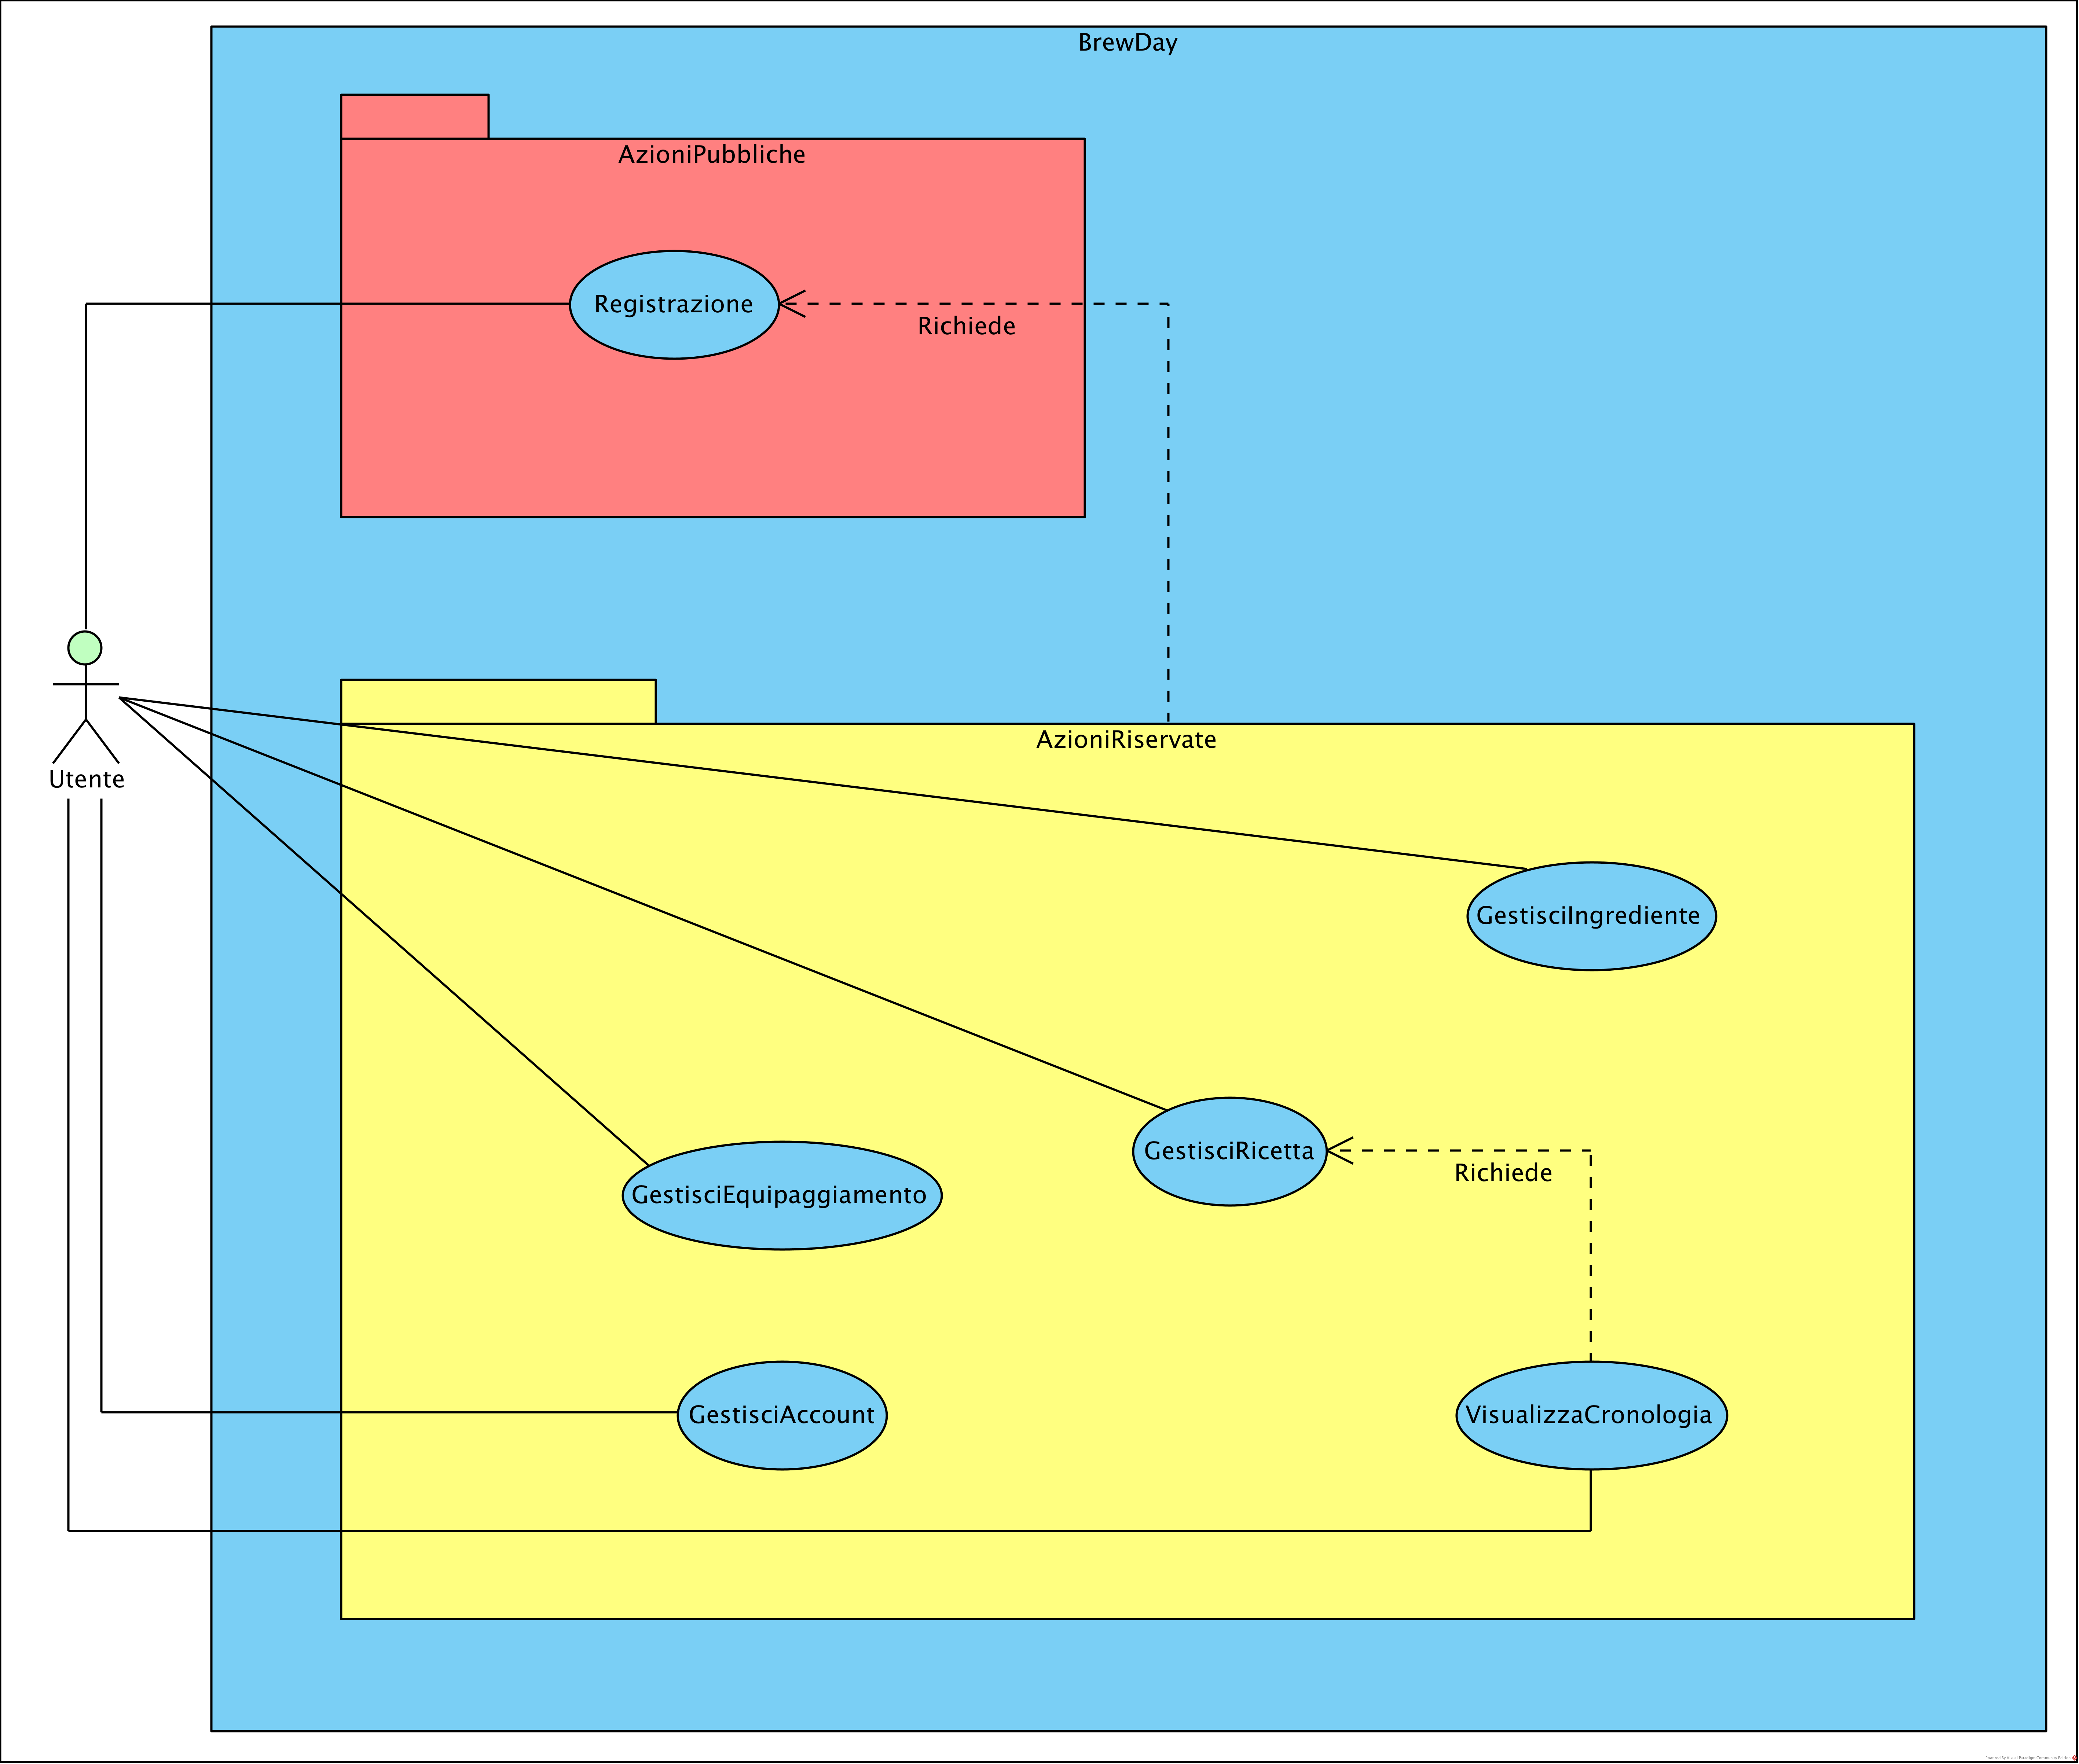
\includegraphics[width=450px]{diagramma_casi_d_uso.png}
\caption{\label{fig:diagramma_casi_d_uso}Diagramma dei casi d'uso}
\end{figure}


\subsection{Modello di Dominio}

\begin{figure}[H]
\centering
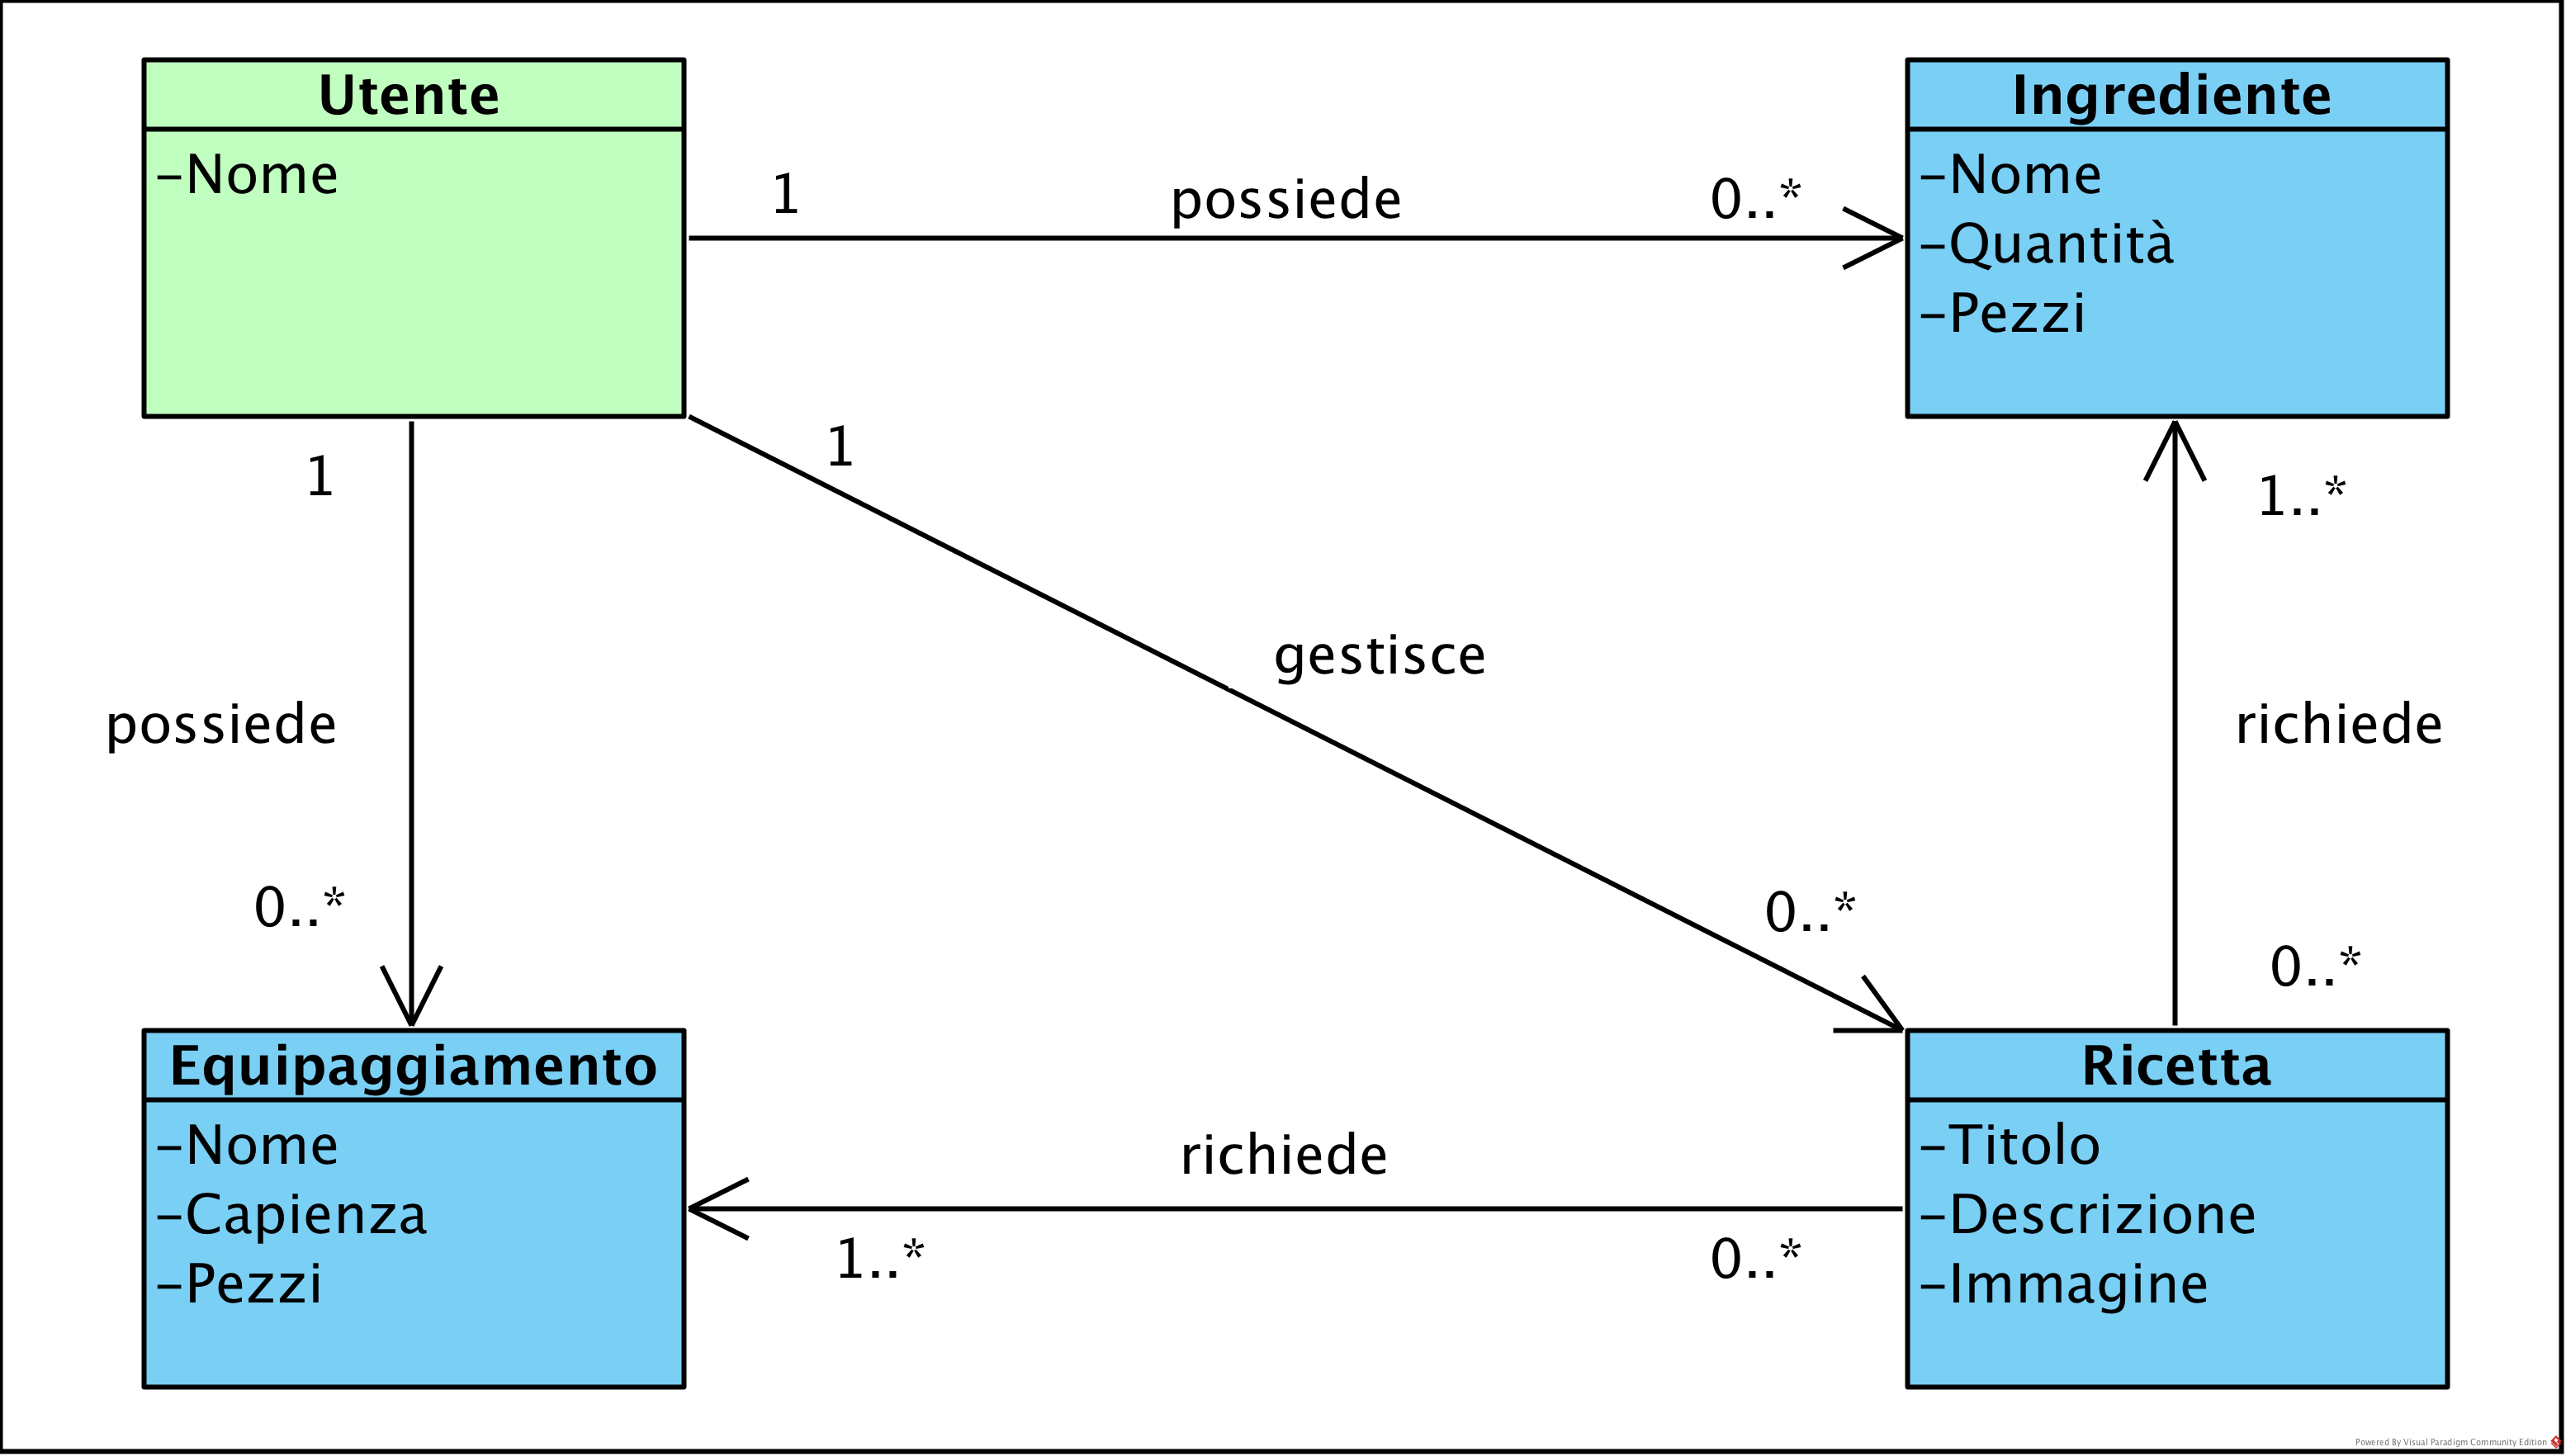
\includegraphics[width=450px]{modello_dominio.png}
\caption{\label{fig:modello_dominio}Modello di Dominio}
\end{figure}



\newpage
\section{Progettazione}

\newpage
\section{Implementazione}


\newpage
\bibliographystyle{alpha}
\bibliography{bibliography}

\begin{abstract}
Your abstract.
\end{abstract}

\end{document}